\documentclass[conference]{IEEEtran}
\usepackage{cite}
\usepackage{amsmath,amssymb,amsfonts}
\usepackage{algorithmic}
\usepackage{graphicx}
\usepackage{textcomp}
\usepackage{xcolor}
\usepackage{tikz}
\usepackage{listings}
\usepackage{booktabs}
\usepackage{multirow}
\usetikzlibrary{shapes.geometric, arrows, positioning, fit, backgrounds}

\lstset{
    language=Python,
    basicstyle=\ttfamily\small,
    keywordstyle=\color{blue},
    commentstyle=\color{green!50!black},
    stringstyle=\color{red},
    frame=single,
    breaklines=true,
    captionpos=b
}

\begin{document}

\title{Autonomous Optimization of ICF Capsule Designs via\\Adversarial Multi-Agent Systems and Reduced-Order Modeling}

\author{\IEEEauthorblockN{Jon Belof}
\IEEEauthorblockA{\textit{Fellow, AI for Science} \\
\textit{Advanced Micro Devices, Inc.}\\
2485 Augustine Dr., Santa Clara, CA 95054\\
jonathan.belof@amd.com}
}

\maketitle

\begin{abstract}
We present a multi-agent system for the autonomous optimization of Inertial Confinement Fusion (ICF) capsule designs under realistic manufacturing uncertainty. The system couples Large Language Model (LLM) reasoning agents with a reduced-order deceleration-phase surrogate model through the Model Context Protocol (MCP), enabling rapid evaluation of thousands of candidate designs. The optimization is formulated as a min-max game between a Design Explorer agent that maximizes fusion yield and a Defect Adversary agent that applies realistic manufacturing perturbations, orchestrated by a Principal Investigator agent. The physics surrogate integrates Hurricane's piston-driven stagnation mechanics with Betti's marginal ignition model, incorporating Spitzer thermal ablation, Gamow thermonuclear burn rates, and linear Rayleigh-Taylor instability growth. We demonstrate that the multi-agent system autonomously navigates the design space along constant-energy manifolds, converging in six rounds from an initial 7.4~MJ baseline to an 11.3~MJ optimized design (53\% yield improvement) that remains robust to mode-1 asymmetries up to $\delta = 0.012$ with RT growth factors below $3.6\times$.
\end{abstract}

%=============================================================================
\section{Introduction}
%=============================================================================

The design of Inertial Confinement Fusion (ICF) targets is a high-dimensional optimization problem in which small perturbations to the capsule geometry or drive symmetry can dramatically degrade performance. High-fidelity radiation hydrodynamics simulations capture the full physics but require $10^4$--$10^6$ CPU-hours per shot, precluding their use in iterative, agent-driven optimization loops. Recent experimental breakthroughs at the National Ignition Facility (NIF)---particularly the N210808 shot that achieved fusion fuel gain exceeding unity \cite{hurricane2014, abu-shawareb2024}---have motivated renewed interest in systematic design-space exploration to identify capsule geometries that are both high-performing and robust to manufacturing variability.

We address this challenge with a multi-agent architecture in which LLM reasoning agents autonomously propose, perturb, evaluate, and iterate on capsule designs. The physics evaluation is performed by a reduced-order surrogate model that captures the essential deceleration-phase dynamics at negligible computational cost ($<1$~second per shot), enabling thousands of evaluations within a single optimization campaign. The agents communicate through the Model Context Protocol (MCP) \cite{mcp2024}, which cleanly decouples the reasoning layer from the simulation execution and provides a natural pathway to future integration with full radiation hydrodynamics codes on HPC clusters.

The optimization is formulated as an adversarial game: a Design Explorer seeks to maximize fusion yield subject to a fixed laser energy budget, while a Defect Adversary applies manufacturing imperfections drawn from current NIF-class fabrication tolerances. This min-max formulation identifies designs that are not merely optimal under ideal conditions but robust to the perturbations that have historically prevented reproducible ignition.

%=============================================================================
\section{Deceleration-Phase Surrogate Model}
\label{sec:model}
%=============================================================================

\subsection{Asymmetric Dual-Piston Formulation}

We model the stagnation phase of an ICF implosion using a zero-dimensional (0D) surrogate that tracks the deceleration, compression, and thermonuclear burn of the hot spot. Following the piston-driven framework of Hurricane \textit{et al.} \cite{hurricane2014}, the imploding shell is treated as a massive piston that decelerates against the rising hot-spot pressure.

To capture mode-1 asymmetry---the dominant low-mode perturbation in NIF implosions arising from laser power imbalance and capsule positioning errors---we decompose the shell into two independent half-shells (``pistons'') with masses
\begin{equation}
M_1 = \frac{M_{sh}}{2}(1 + \delta), \qquad M_2 = \frac{M_{sh}}{2}(1 - \delta)
\label{eq:masses}
\end{equation}
where $M_{sh}$ is the total shell mass and $\delta \in [0, 0.15]$ is the mode-1 asymmetry fraction. Each piston has independent position $R_i$ and velocity $v_i$ governed by
\begin{equation}
\frac{dR_i}{dt} = v_i, \qquad \frac{dv_i}{dt} = \frac{A_{eff} \, P_{hs}}{M_i}
\label{eq:piston}
\end{equation}
where $A_{eff} = 4\pi R_{eff}^2$ is the effective hot-spot surface area, $R_{eff} = (R_1 + R_2)/2$ is the mean radius, and $P_{hs}$ is the hot-spot pressure derived from the internal energy via an ideal gas equation of state:
\begin{equation}
P_{hs} = \frac{2}{3} \frac{E_{hs}}{V}, \qquad V = \frac{4}{3}\pi R_{eff}^3
\label{eq:pressure}
\end{equation}

The asymmetry $\delta$ introduces differential deceleration of the two pistons: the lighter half-shell ($M_2$) decelerates faster, producing asymmetric stagnation radii and directing kinetic energy into residual motion rather than compression work. This residual kinetic energy
\begin{equation}
E_{RKE} = \frac{1}{2}M_1 v_1^2 + \frac{1}{2}M_2 v_2^2
\label{eq:rke}
\end{equation}
represents energy unavailable for hot-spot heating and directly quantifies the yield penalty from mode-1 drive asymmetry.

\subsection{Hot-Spot Energy Balance}

The hot-spot internal energy evolves according to
\begin{equation}
\frac{dE_{hs}}{dt} = -P_{hs}\frac{dV}{dt} + W_\alpha - W_{rad}
\label{eq:energy}
\end{equation}
where the three terms represent compressive $PdV$ work (the dominant heating source during deceleration), alpha-particle self-heating, and radiative losses, respectively.

\subsubsection{Thermonuclear Burn Rate}
The DT fusion reaction rate density is computed from the ion number density $n_i = \rho_{hs}/m_{DT}$ (where $m_{DT} = 2.5\,m_p$) using the NRL Plasma Formulary parametrization of the Gamow peak cross-section \cite{nrl2019}:
\begin{equation}
\langle\sigma v\rangle = 3.68 \times 10^{-12} \, T_{keV}^{-2/3} \exp\!\left(-19.94 \, T_{keV}^{-1/3}\right) \;\text{cm}^3/\text{s}
\label{eq:sigmav}
\end{equation}
This parametrization is preferred over the Bosch-Hale fit \cite{bosch1992} because it remains numerically stable across the full temperature range encountered during the explosive alpha-heating phase, avoiding the mathematical stiffness introduced by the polynomial denominator in the Bosch-Hale expression. The volumetric reaction rate is $R_{rxn} = (n_f/2)^2 \langle\sigma v\rangle \cdot V$, where $n_f$ is the fuel ion density (accounting for the evolving fuel fraction within the hot spot), and the alpha-heating power is
\begin{equation}
W_\alpha = R_{rxn} \cdot E_\alpha, \qquad E_\alpha = 3.5\;\text{MeV}
\label{eq:alpha}
\end{equation}

\subsubsection{Radiative Losses}
Bremsstrahlung radiation is modeled as
\begin{equation}
W_{rad}^{vol} = 5.34 \times 10^{-37} \, n_i^2 \sqrt{T_{keV}} \cdot V \;\;\text{[W]}
\label{eq:bremsstrahlung}
\end{equation}
which is capped by the blackbody limit $W_{bb} = \sigma_{SB} T^4 \cdot 4\pi R_{eff}^2$ to prevent unphysical radiative losses at extreme temperatures. The effective radiative loss is $W_{rad} = \min(W_{rad}^{vol},\, W_{bb})$.

\subsection{Spitzer Ablation and Hot-Spot Mass Evolution}

Following the Betti marginal ignition model \cite{betti2002}, we couple the shell dynamics to the hot-spot mass through Spitzer electron thermal conduction. As the hot spot heats during compression, a thermal conduction front ablates material from the inner surface of the cold shell into the hot spot:
\begin{equation}
\frac{dM_{hs}}{dt} = C_{abl} \, R_{eff} \, T_{keV}^{5/2}
\label{eq:ablation}
\end{equation}
where $C_{abl}$ is the ablation coefficient and the $T^{5/2}$ dependence reflects the Spitzer thermal conductivity of a fully ionized plasma. This ablation is activated only when $T > 0.5$~keV to prevent unphysical mass injection at early, cold times. The ablated mass replenishes the DT fuel supply within the hot spot, while burned fuel is consumed at rate $\dot{M}_{fuel,burn} = R_{rxn} \cdot 2\,m_{DT}$.

This dynamic mass coupling is physically important: it creates a positive feedback loop in which compression heating drives ablation, which increases the hot-spot density and hence the burn rate, which produces more alpha heating. This feedback is the mechanism by which marginal ignition transitions to propagating burn.

\subsection{Rayleigh-Taylor Instability Growth}

Hydrodynamic instabilities at the shell-hot-spot interface are tracked via the linear Rayleigh-Taylor (RT) growth rate. During deceleration ($g_{eff} > 0$), small perturbations at mode number $\ell$ grow as
\begin{equation}
\frac{d\xi}{dt} = \sqrt{k \, g_{eff}}, \qquad k = \frac{\ell}{R_{eff}}
\label{eq:rt}
\end{equation}
where $g_{eff} = (a_1 + a_2)/2$ is the mean deceleration and $\xi$ is the integrated growth exponent. The physical perturbation amplitude at stagnation is $A_{stag} = A_0 \exp(\xi)$, where $A_0$ is the initial surface roughness. When the RT amplitude approaches the shell thickness, the shell integrity is compromised and confinement is lost---a primary failure mode in under-performing NIF shots.

\subsection{State Vector and Numerical Integration}

The complete system is a 9-component ODE:
\begin{equation}
\mathbf{y} = \left[R_1,\, v_1,\, R_2,\, v_2,\, E_{hs},\, Y,\, \xi,\, M_{fuel},\, M_{hs}\right]
\label{eq:state}
\end{equation}
where $Y$ is the cumulative fusion yield ($dY/dt = 5\,W_\alpha$, the factor of 5 accounting for total fusion energy per alpha particle). The system is integrated using the \texttt{Radau} implicit Runge-Kutta method \cite{hairer1996} with adaptive stepping, which is essential for resolving the extreme stiffness introduced by the alpha-heating spike at ignition. Typical integration spans 0.6~ns with maximum step size $10^{-12}$~s and absolute tolerance $10^{-8}$.

%=============================================================================
\section{Adversarial Optimization Formulation}
\label{sec:optimization}
%=============================================================================

\subsection{Min-Max Game Structure}

The design optimization is formulated as a two-player adversarial game:
\begin{equation}
\max_{\mathbf{x} \in \mathcal{X}} \;\; \min_{\mathbf{d} \in \mathcal{D}} \;\; Y(\mathbf{x}, \mathbf{d})
\label{eq:minmax}
\end{equation}
where $\mathbf{x} = (R_0, v_0, T_0, M_{sh}, M_{hs})$ are the design variables controlled by the Explorer, $\mathbf{d} = (\delta, \ell, A_0)$ are the defect parameters controlled by the Adversary, and $Y$ is the total fusion yield.

\subsection{Energy Constraint}

The design space is constrained by the available laser energy. The kinetic energy of the imploding shell at the onset of deceleration is related to the laser energy through a hydrodynamic coupling efficiency $\eta$:
\begin{equation}
E_k = \frac{1}{2}M_{sh} v_0^2 = \eta \, E_{laser}
\label{eq:energy_constraint}
\end{equation}
For NIF-class indirect-drive implosions, $\eta \approx 0.015$; a $3$~MJ laser then gives a kinetic energy budget of $E_k = 45$~kJ. The laser energy is not fixed: it is parsed from the user's request and the corresponding budget is computed and supplied to the agents at the start of each campaign, so the same machinery scans the full range from sub-MJ to multi-MJ drives. This constraint defines a one-dimensional manifold in $(M_{sh}, v_0)$ space: increasing shell mass requires decreasing implosion velocity, and vice versa. The fundamental tradeoff is between \textit{fuel inventory} (more mass to burn) and \textit{implosion vigor} (higher velocity for stronger compression and higher stagnation temperature).

\subsection{Defect Bounds}

The Adversary's parameter space is bounded by current manufacturing tolerances for NIF-class targets:
\begin{itemize}
    \item \textbf{Mode-1 asymmetry} $\delta \in [0, 0.15]$: arising from laser power imbalance, beam pointing errors, and capsule offset within the hohlraum. Typical NIF values are $\delta \approx 0.02$--$0.05$; values above $0.10$ represent severe drive asymmetry.
    \item \textbf{RT mode number} $\ell \in [2, 40]$: the dominant perturbation wavelength, with low modes ($\ell < 10$) from drive asymmetry and high modes ($\ell > 20$) from surface roughness and microstructure.
    \item \textbf{Surface roughness} $A_0 \in [0, 3\,\mu\text{m}]$: the initial perturbation amplitude at the inner shell surface, set by fabrication quality. Current NIF capsules achieve $A_0 \approx 0.1$--$1.0\,\mu$m.
\end{itemize}

These bounds are enforced at the server level: parameter values submitted outside these ranges are clamped and a warning is returned to the requesting agent, providing feedback that guides subsequent proposals.

%=============================================================================
\section{Multi-Agent Architecture}
\label{sec:agents}
%=============================================================================

\subsection{Agent Roles and Communication}

The system comprises four agents coordinated through the AutoGen framework \cite{autogen2023} using structured group chat with constrained speaker transitions:

\begin{enumerate}
    \item \textbf{Principal Investigator (PI)}: The orchestrator agent, implemented on a frontier LLM. It coordinates the optimization campaign by sequentially engaging the Explorer and Adversary, validates the energy constraint (Eq.~\ref{eq:energy_constraint}), invokes the simulation tool, evaluates results against ignition criteria (yield $> 1$~MJ, stagnation pressure $> 100$~Gbar, RT amplification $< 1000\times$), and decides whether to iterate or terminate. The PI is the \textit{only} agent authorized to call the simulation tool.

    \item \textbf{Design Explorer}: Proposes capsule design parameters $\mathbf{x}$ to maximize yield. This agent is intended to run on a domain-specific LLM fine-tuned on high-energy-density-physics literature, enabling physics-informed design intuition beyond what is available from general-purpose models. In the local deployment described in Section~\ref{sec:deployment}, all agents are served by such a model (\texttt{gptoss-20b-hedp}, a 20B-parameter open-weight model fine-tuned on HEDP papers). It receives feedback from prior simulation results and adjusts parameters along the constant-energy manifold.

    \item \textbf{Defect Adversary}: Proposes manufacturing defect parameters $\mathbf{d}$ to stress-test the Explorer's designs. It follows a systematic strategy: probing individual defect modes in early rounds to identify the design's primary sensitivity, then combining the most damaging perturbations in later rounds.

    \item \textbf{User Proxy}: An execution bridge that receives tool calls from the PI and dispatches them to the MCP server. It performs no reasoning and does not modify parameters.
\end{enumerate}

\subsection{Speaker Transition Constraints}

To prevent degenerate conversation patterns (infinite loops, role confusion, agents attempting unauthorized tool calls), the group chat enforces hard speaker transition constraints:

\begin{center}
\begin{tabular}{ll}
\toprule
\textbf{After speaker} & \textbf{Allowed next speakers} \\
\midrule
User Proxy & PI only \\
PI & Explorer, Adversary, or User Proxy \\
Explorer & PI only \\
Adversary & PI only \\
\bottomrule
\end{tabular}
\end{center}

This ensures a hub-and-spoke topology: all information flows through the PI, which maintains global state and enforces the optimization protocol. The Explorer and Adversary cannot communicate directly or invoke tools.

\subsection{MCP Tool Server}

The physics surrogate is served as an MCP tool via the FastMCP framework. The tool interface accepts all 8 physical parameters in SI units and returns structured simulation results (stagnation metrics, fusion yield, burn fraction, residual kinetic energy, RT amplification). The MCP server enforces hard physical bounds on all input parameters (Table~\ref{tab:bounds}), clamping out-of-range values and returning warnings to the calling agent. This server-side validation is essential because LLM agents frequently propose values outside specified bounds despite prompt instructions.

\begin{table}[htbp]
\caption{Parameter Bounds Enforced by the MCP Server}
\label{tab:bounds}
\centering
\begin{tabular}{llll}
\toprule
\textbf{Parameter} & \textbf{Min} & \textbf{Max} & \textbf{Units} \\
\midrule
$R_0$ & $3 \times 10^{-5}$ & $5 \times 10^{-4}$ & m \\
$v_0$ & $-8 \times 10^{5}$ & $-1 \times 10^{5}$ & m/s \\
$T_0$ & 0.1 & 10.0 & keV \\
$M_{sh}$ & $10^{-8}$ & $2 \times 10^{-6}$ & kg \\
$M_{hs}$ & $10^{-9}$ & $10^{-7}$ & kg \\
$\delta$ & 0.0 & 0.15 & --- \\
$\ell$ & 2 & 40 & --- \\
$A_0$ & 0.0 & $3 \times 10^{-6}$ & m \\
\bottomrule
\end{tabular}
\end{table}

The decoupling of physics execution from agent reasoning via MCP is architecturally significant: it allows the simulation backend to be replaced transparently---from the 0D surrogate used here, to a 1D Lagrangian hydrocode, to a full 2D/3D radiation hydrodynamics code on an HPC cluster---without modifying any agent logic.

\begin{figure}[htbp]
\centering
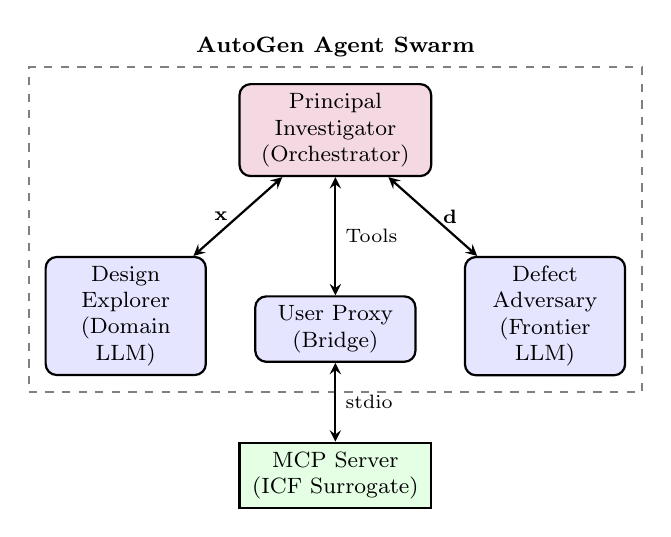
\begin{tikzpicture}[
    node distance=1.0cm and 0.4cm,
    box/.style={rectangle, draw=black, thick, fill=blue!10, text width=1.8cm, align=center, minimum height=0.8cm, rounded corners, font=\footnotesize},
    tool/.style={rectangle, draw=black, thick, fill=green!10, text width=2.2cm, align=center, minimum height=0.8cm, font=\footnotesize},
    arrow/.style={thick, ->, >=stealth}
]

\node (pi) [box, fill=purple!15, text width=2.2cm] {Principal\\Investigator\\(Orchestrator)};
\node (explorer) [box, below left=of pi] {Design\\Explorer\\(Domain LLM)};
\node (adversary) [box, below right=of pi] {Defect\\Adversary\\(Frontier LLM)};
\node (proxy) [box, below=1.5cm of pi] {User Proxy\\(Bridge)};
\node (mcp) [tool, below=of proxy] {MCP Server\\(ICF Surrogate)};

\draw [arrow, <->] (pi) -- (explorer) node[midway, left, font=\scriptsize] {$\mathbf{x}$};
\draw [arrow, <->] (pi) -- (adversary) node[midway, right, font=\scriptsize] {$\mathbf{d}$};
\draw [arrow, <->] (pi) -- (proxy) node[midway, right, font=\scriptsize] {Tools};
\draw [arrow, <->] (proxy) -- (mcp) node[midway, right, font=\scriptsize] {stdio};

\begin{scope}[on background layer]
    \node [draw=gray, dashed, thick, fit=(pi) (explorer) (adversary) (proxy), inner sep=0.2cm, label=above:{\footnotesize\textbf{AutoGen Agent Swarm}}] {};
\end{scope}

\end{tikzpicture}
\caption{Architecture of the 4-agent system. The PI orchestrates the adversarial game, delegating design proposals ($\mathbf{x}$) to the Explorer and defect proposals ($\mathbf{d}$) to the Adversary. Only the PI invokes the MCP physics server through the User Proxy.}
\label{fig:architecture}
\end{figure}

\subsection{Deployment and Backends}
\label{sec:deployment}

The system supports two interchangeable LLM backends, selected at launch. The first is a frontier cloud model accessed through a hosted API, in which the PI invokes the simulation through the framework's native tool-calling interface. The second is a fully local deployment in which an open-weight model fine-tuned on HEDP literature (\texttt{gptoss-20b-hedp}, 20B parameters) is served through a high-throughput inference engine (vLLM) on AMD Instinct GPUs, exposing an OpenAI-compatible endpoint. The local deployment is significant for security-sensitive design work, where sending capsule parameters to an external service is undesirable: the entire reasoning--simulation loop runs on-premises. The OpenAI-compatible backend is not restricted to on-premises servers---the same interface drives a \emph{remote} hosted endpoint (for example an AIMS/LUX-hosted \texttt{gpt-oss-120b}) with no code changes, so the deployment scales from a single local GPU to a shared inference cluster. In all cases a single shared model backs every agent role; the architecture permits distinct per-role models (e.g.\ a domain-tuned Explorer alongside a frontier PI), but the reference implementation uses one model configured entirely through environment variables, keeping credentials out of the source tree.

\subsection{Robustness Layer for Open-Weight Models}

Small open-weight models are markedly less reliable than frontier models at the structured behaviors the orchestration depends on. Six mechanisms make the deployment robust:

\begin{enumerate}
    \item \textbf{Text-based tool invocation.} Rather than relying on a structured tool-call API, the PI emits a plain-text directive (\texttt{RUN\_SIMULATION: R0=..., v0=..., ...}) that a parser intercepts, validates, executes against the MCP server, and replaces with the returned metrics. A markdown-tolerant regular expression handles the formatting variability typical of these models. This sidesteps the brittle and architecture-specific structured-output tokens that otherwise cause server-side parse failures.
    \item \textbf{Deterministic speaker scheduling.} Speaker selection follows a fixed cycle (PI $\rightarrow$ Explorer $\rightarrow$ PI $\rightarrow$ Adversary $\rightarrow$ PI) rather than an LLM-driven selector, eliminating the malformed-selection errors and degenerate loops that small models produce when asked to choose the next speaker.
    \item \textbf{Response sanitization.} A wrapper on the model client strips stray tool-call artifacts and substitutes empty strings for null content before any downstream processing, preventing exceptions from non-conforming responses.
    \item \textbf{Bounded context.} A history-trimming hook caps what each agent sees to the campaign's opening message (which carries the energy budget) plus the most recent exchanges, so a long campaign cannot overflow the model's context window.
    \item \textbf{Deterministic convergence.} The stopping decision is computed in code from the recorded simulation yields (the campaign halts once the best yield improves by less than 5\% for two consecutive simulations) rather than trusting the model to emit a termination signal on schedule. This guarantees a clean, explainable end to every campaign even when the model does not follow the stopping protocol.
    \item \textbf{Bounded requests.} Every model call carries a per-request timeout with automatic retries, so a slow or stalled generation on a remote endpoint---which would otherwise block the whole campaign indefinitely---is bounded and recovered rather than hanging the run.
\end{enumerate}

\subsection{Operational Modes and Interface}

The agent swarm is served through a Gradio web interface that provides real-time visibility into the multi-agent conversation. The group chat runs in a background thread while a generator polls the shared message list, streaming each agent's contribution to the browser as it is produced---the Explorer's design rationale, the Adversary's perturbation strategy, and the PI's evaluation of each simulation. A user request is routed by intent into one of four modes:

\begin{itemize}
    \item \textbf{Single design campaign:} one optimization campaign at a requested laser energy, streamed live.
    \item \textbf{Laser-energy sweep:} one full campaign per energy point, producing a plot of fusion yield versus laser energy. Each point reports the \emph{mean} yield over the campaign's simulations with $\pm 1\sigma$ error bars; the variance is itself a diagnostic, growing where the design space straddles the ignition threshold (Section~\ref{sec:results}). The energy grid is parsed from natural language and supports multiple range segments with independent step sizes (e.g.\ fine spacing across the ignition cliff and coarse spacing across the high-yield plateau).
    \item \textbf{Simulation media:} the best design from a campaign is rendered as an animation of the imploding density field and as diagnostic time-history traces.
    \item \textbf{Interactive analysis (debrief):} once at least one campaign has run, the user can pose natural-language questions about the results---\textit{why} a design won, \textit{how} robust it is to defects, or \textit{which} parameter dominated---and receive a written analysis rather than a new simulation.
\end{itemize}

Each campaign is bounded by a maximum number of agent rounds and a yield-plateau stopping criterion (Section~\ref{sec:agents} prompt protocol). When a campaign yields no valid simulation, a physically reasonable fallback design at the target energy keeps the sweep and media outputs populated.

\subsection{Conversational Debrief of Campaign Results}

The first three modes are generative---they spend simulation budget to produce new designs. The fourth is interpretive. Every campaign's structured outcome (the best design and its yield, every sampled design with its eight parameters and resulting yield, the mean/$\sigma$ statistics, any sweep curve, and rendered-media references) is retained in a session-scoped store that persists across conversational turns. When the user's message is a question about prior results rather than a request to run something, an intent router dispatches it to a dedicated \emph{conversational PI} agent: the same frontier LLM as the orchestrating PI but operating from a debrief prompt with no simulation tool and no authority to alter the design. It is supplied the serialized result store as context and answers strictly from that data, declining and suggesting a follow-up campaign when the necessary information is absent. The exchange carries multi-turn memory, so follow-up questions retain context. The router separates the two intents with a keyword heuristic: explicit run verbs (\texttt{optimize}, \texttt{sweep}, \texttt{render a movie}) and energy-bearing requests start a campaign, while interrogatives and analysis verbs (\texttt{why}, \texttt{how}, \texttt{compare}, \texttt{explain}, \texttt{robust}) route to the debrief agent. This converts the system from a fire-and-forget optimizer into an interactive design assistant, with the human able to interrogate the rationale behind a result without re-running the swarm.

%=============================================================================
\section{Results}
\label{sec:results}
%=============================================================================

\subsection{Design Space Exploration Along Constant-Energy Manifolds}

Table~\ref{tab:ke_sweep} presents a systematic exploration of the $(M_{sh}, v_0)$ tradeoff along the 45~kJ constant-energy manifold at fixed $R_0 = 150\,\mu$m, $T_0 = 1.0$~keV, $M_{hs} = 5$~ng, and zero defects. Yield increases monotonically with shell mass (at correspondingly lower velocity), from 4.2~MJ at $M_{sh} = 0.1\,\mu$g to 11.4~MJ at $M_{sh} = 1.0\,\mu$g. This reflects the dominant role of fuel inventory: more DT mass produces more burn even at reduced implosion velocity, provided the stagnation conditions remain above the ignition threshold.

\begin{table}[htbp]
\caption{Design Exploration Along the 45~kJ Energy Manifold}
\label{tab:ke_sweep}
\centering
\begin{tabular}{cccc}
\toprule
$M_{sh}$ [$\mu$g] & $|v_0|$ [km/s] & Yield [MJ] & Burn [\%] \\
\midrule
0.10 & 949 & 4.24 & 15.0 \\
0.20 & 671 & 5.93 & 16.0 \\
0.25 & 600 & 6.56 & 16.2 \\
0.36 & 500 & 7.70 & 16.5 \\
0.50 & 424 & 8.84 & 16.6 \\
0.80 & 335 & 10.6 & 16.6 \\
1.00 & 300 & 11.4 & 16.6 \\
\bottomrule
\end{tabular}
\end{table}

The burn fraction saturates near 16.6\%, consistent with the Betti marginal ignition scaling in which the burn-up fraction is primarily determined by the areal density at stagnation rather than the total fuel mass \cite{betti2002}.

\subsection{Sensitivity to Initial Conditions}

The surrogate exhibits sharp ignition cliffs in several parameters, reflecting the threshold nature of thermonuclear ignition. At fixed baseline conditions ($M_{sh} = 0.25\,\mu$g, $v_0 = -450$~km/s, $\delta = 0.05$):

\begin{itemize}
    \item \textbf{Stagnation radius}: Yield drops from 7.0~MJ at $R_0 = 150\,\mu$m to 0.06~MJ at $R_0 = 200\,\mu$m---a $100\times$ reduction from a 33\% increase in radius. Larger $R_0$ reduces the convergence ratio, producing insufficient compression for ignition.

    \item \textbf{Initial temperature}: Yield peaks at $T_0 \approx 1.0$~keV and drops precipitously above 1.5~keV. Higher initial temperatures reduce the density at fixed pressure, weakening the compressive $PdV$ heating during deceleration.

    \item \textbf{Hot-spot mass}: Yield peaks near $M_{hs} = 5$~ng and drops to near zero above 10~ng. Excessive initial hot-spot mass dilutes the temperature at fixed energy, preventing the plasma from reaching the $\sim$$5$~keV threshold where alpha heating becomes dominant.
\end{itemize}

These cliffs define the boundaries of the ignition region and constrain the Explorer's viable design space.

\subsection{Robustness to Mode-1 Asymmetry}

Table~\ref{tab:delta} compares the defect sensitivity of three designs along the 45~kJ manifold under increasing mode-1 asymmetry with $\ell = 20$ and $A_0 = 2\,\mu$m.

\begin{table}[htbp]
\caption{Yield and Residual KE vs.\ Mode-1 Asymmetry $\delta$}
\label{tab:delta}
\centering
\begin{tabular}{ccccc}
\toprule
\multirow{2}{*}{$\delta$} & \multicolumn{2}{c}{Baseline ($0.25\,\mu$g)} & \multicolumn{2}{c}{Optimized ($0.36\,\mu$g)} \\
\cmidrule(lr){2-3} \cmidrule(lr){4-5}
& $Y$ [MJ] & $E_{RKE}$ [J] & $Y$ [MJ] & $E_{RKE}$ [J] \\
\midrule
0.00 & 7.02 & 6.8 & 8.17 & 1918 \\
0.04 & 7.02 & 49 & 8.16 & 2036 \\
0.08 & 7.01 & 178 & 8.15 & 2389 \\
0.12 & 7.00 & 395 & 8.12 & 2972 \\
0.15 & 6.99 & 617 & 8.10 & 6315 \\
\bottomrule
\end{tabular}
\end{table}

Both designs maintain ignition across the full range of physically realistic asymmetries. The baseline design shows remarkable stability: yield degrades by only 0.4\% ($\Delta Y = 0.03$~MJ) even at the maximum asymmetry $\delta = 0.15$. The optimized design achieves 16\% higher absolute yield but exhibits larger residual kinetic energy, indicating less efficient energy coupling at stagnation. Under worst-case combined defects ($\delta = 0.12$, $\ell = 20$, $A_0 = 2\,\mu$m), the high-mass design ($M_{sh} = 1.0\,\mu$g, $v_0 = 300$~km/s) achieves the highest yield of 11.4~MJ with modest residual KE of 684~J.

\subsection{Rayleigh-Taylor Amplification}

Table~\ref{tab:rt} shows the RT amplification factor at stagnation as a function of perturbation mode number for the baseline design. The exponential growth characteristic of the linear RT instability produces amplification factors exceeding $10^3$ at $\ell = 30$, indicating that high-mode surface perturbations can grow to amplitudes comparable to the shell thickness during deceleration. In the current 0D model, RT growth is tracked diagnostically and does not feed back into the yield calculation; coupling RT-induced mix into the hot-spot energy balance is a planned extension.

\begin{table}[htbp]
\caption{RT Amplification Factor vs.\ Mode Number}
\label{tab:rt}
\centering
\begin{tabular}{cc}
\toprule
Mode $\ell$ & Amplification $e^\xi$ \\
\midrule
2 & $6.1\times$ \\
5 & $17\times$ \\
10 & $57\times$ \\
15 & $142\times$ \\
20 & $305\times$ \\
30 & $1104\times$ \\
40 & $3262\times$ \\
\bottomrule
\end{tabular}
\end{table}

\subsection{Autonomous Optimization Campaign}

To demonstrate the end-to-end system, we executed a complete adversarial optimization campaign using the domain-specific \texttt{gptoss-20b-hedp} model (a 20B parameter LLM fine-tuned on HEDP literature) served via vLLM on AMD MI355X GPUs. The campaign proceeded autonomously through six rounds of design iteration, defect testing, and parameter refinement, converging on a high-yield design robust to manufacturing defects. Table~\ref{tab:campaign} summarizes the optimization trajectory.

\begin{table}[htbp]
\caption{Autonomous Agent Optimization Campaign}
\label{tab:campaign}
\centering
\begin{tabular}{clccc}
\toprule
Round & Design Change & $\delta$ & $Y$ [MJ] & $\Delta Y$ \\
\midrule
1 & Baseline ($M_{sh}\!=\!0.265\,\mu$g, & 0.04 & 7.4 & --- \\
  & $|v_0|\!=\!585$~km/s) & & & \\
2 & High-mode stress test & 0.015 & 5.8 & $-22\%$ \\
3 & Heavier shell ($M_{sh}\!=\!0.28\,\mu$g, & 0.02 & 9.3 & $+60\%$ \\
  & $|v_0|\!=\!600$~km/s, $T_0\!=\!1.8$~keV) & & & \\
4 & Tighter defect ($\delta\!=\!0.012$) & 0.012 & 9.8 & $+5.4\%$ \\
5 & Light shell, high velocity & 0.01 & 11.3 & $+15\%$ \\
  & ($M_{sh}\!=\!0.245\,\mu$g, $|v_0|\!=\!610$~km/s) & & & \\
6 & Hot-spot boost ($T_0\!=\!2.2$~keV) & 0.01 & 11.3 & $<1\%$ \\
\bottomrule
\end{tabular}
\end{table}

Several features of the agent behavior merit discussion:

\textbf{Adversary strategy.} The Defect Adversary autonomously varied its perturbation strategy across rounds, first applying moderate mode-1 asymmetry ($\delta = 0.04$, $\ell = 10$), then switching to a high-mode surface roughness attack ($\delta = 0.015$, $\ell = 30$, $A_0 = 2\,\mu$m) that reduced yield by 22\%. This systematic probing---low-mode first, then high-mode---was specified in the agent's system prompt but the specific parameter choices were determined autonomously by the LLM.

\textbf{Explorer adaptation.} After the high-mode defect reduced yield to 5.8~MJ in Round~2, the Design Explorer autonomously shifted to a heavier-shell, higher-velocity design point on the constant-energy manifold, recovering yield to 9.3~MJ in Round~3. The Explorer then proposed a ``light shell, high velocity'' variant that traded shell mass for implosion velocity, reaching 11.3~MJ---a 53\% improvement over the initial baseline.

\textbf{Convergence.} The PI agent tracked yield improvements across rounds and initiated a defect-sensitivity sweep when the yield plateau was approached. The sweep revealed that the optimized design maintains $Y > 10$~MJ for $\delta \leq 0.012$ with RT growth factors below $3.6\times$, establishing a quantitative stability margin. The campaign terminated when yield improvement fell below the 5\% threshold for two consecutive rounds.

\textbf{Defect-sensitivity of the final design.} Table~\ref{tab:agent_sweep} presents the defect sweep conducted autonomously by the agent system for the optimized design ($M_{sh} = 0.245\,\mu$g, $|v_0| = 610$~km/s, $T_0 = 2.0$~keV).

\begin{table}[htbp]
\caption{Agent-Directed Defect Sweep of Optimized Design}
\label{tab:agent_sweep}
\centering
\begin{tabular}{cccc}
\toprule
$\delta$ & Yield [MJ] & $P_{stag}$ [Mbar] & RT Growth \\
\midrule
0.008 & 11.7 & 1.92 & $2.7\times$ \\
0.010 & 11.3 & 1.90 & $3.1\times$ \\
0.012 & 10.8 & 1.88 & $3.6\times$ \\
\bottomrule
\end{tabular}
\end{table}

The final recommended design achieves 11.3~MJ at $\delta = 0.01$ with comfortable stability margin, representing a $53\%$ yield improvement over the initial N210808-inspired baseline within the same 45~kJ kinetic energy budget.

%=============================================================================
\section{Discussion}
%=============================================================================

The results demonstrate that the multi-agent system autonomously discovers the key design tradeoffs in ICF. The parametric sweeps (Tables~\ref{tab:ke_sweep}--\ref{tab:rt}) establish the structure of the design space, while the autonomous campaign (Tables~\ref{tab:campaign}--\ref{tab:agent_sweep}) shows the agents navigating this space in real time. Notably, the agents autonomously discovered the velocity-for-mass tradeoff along the constant-energy manifold: after a high-mode defect reduced yield by 22\% in Round~2, the Explorer shifted to a lighter, faster shell that recovered and exceeded the original yield, ultimately achieving an 11.3~MJ design robust to $\delta \leq 0.012$ --- a 53\% improvement over the initial baseline within the same energy budget.

Several limitations of the current surrogate should be noted. First, the RT instability is tracked but does not degrade confinement or inject cold material into the hot spot; incorporating RT-induced mix would sharpen the ignition cliff at high mode numbers and penalize designs with large convergence ratios. Second, the model assumes a single-temperature plasma ($T_i \approx T_e$), neglecting ion-electron equilibration dynamics that are important at early times. Third, the 0D geometry cannot capture multidimensional effects such as jet formation from mode-1 asymmetry or the development of turbulent mix layers. Despite these limitations, the surrogate correctly reproduces the qualitative scaling of yield with implosion velocity, shell mass, and asymmetry observed in NIF experiments.

The MCP-based architecture provides a clear upgrade path: replacing the surrogate with a 1D Lagrangian hydrocode (e.g., LILAC or HYDRA in 1D mode) would capture shock timing, ablation-front RT growth, and equation-of-state effects while remaining fast enough for agent-driven optimization. Integration with full 2D/3D radiation hydrodynamics codes would require asynchronous job submission to HPC clusters, but the MCP protocol supports this naturally through its tool-call abstraction.

%=============================================================================
\section{Conclusions}
%=============================================================================

We have presented a multi-agent system that autonomously optimizes ICF capsule designs under adversarial manufacturing uncertainty. The key contributions are:

\begin{enumerate}
    \item A deceleration-phase surrogate model combining Hurricane's dual-piston stagnation mechanics with Betti's Spitzer ablation and marginal ignition physics, integrated as a stiff 9-component ODE system.
    \item An adversarial min-max optimization formulation (Eq.~\ref{eq:minmax}) that discovers designs robust to mode-1 asymmetry, RT instability, and surface roughness within NIF-class manufacturing tolerances.
    \item A 4-agent architecture with constrained speaker transitions and server-enforced parameter bounds, addressing practical challenges of LLM-driven optimization (unit confusion, role drift, out-of-bounds proposals).
    \item Demonstration of autonomous convergence: agents navigate the $(M_{sh}, v_0)$ manifold over six rounds, improving yield from 7.4~MJ to 11.3~MJ (53\% gain) while maintaining robustness to $\delta \leq 0.012$ asymmetry, with yield-plateau stopping criteria terminating the campaign automatically.
    \item An interactive debrief mode in which a tool-free conversational instance of the PI reasons over a persistent, session-scoped store of campaign results, allowing the human to interrogate the rationale and robustness of any completed design without re-running the swarm.
\end{enumerate}

The MCP-based decoupling of reasoning agents from physics execution provides a natural pathway to scaling this approach to high-fidelity radiation hydrodynamics simulations on HPC clusters, transforming the human-in-the-loop design bottleneck into an automated, adversarially robust optimization cycle.

\begin{thebibliography}{00}
\bibitem{hurricane2014} O. A. Hurricane \textit{et al.}, ``Fuel gain exceeding unity in an inertially confined fusion implosion,'' \textit{Nature}, vol. 506, pp. 343--348, 2014.
\bibitem{abu-shawareb2024} H. Abu-Shawareb \textit{et al.}, ``Achievement of target gain larger than unity in an inertial fusion experiment,'' \textit{Phys. Rev. Lett.}, vol. 132, p. 065102, 2024.
\bibitem{betti2002} R. Betti \textit{et al.}, ``Deceleration phase of inertial confinement fusion implosions,'' \textit{Phys. Plasmas}, vol. 9, no. 5, pp. 2277--2286, 2002.
\bibitem{nrl2019} J. D. Huba, \textit{NRL Plasma Formulary}, Naval Research Laboratory, Washington, DC, 2019.
\bibitem{bosch1992} H.-S. Bosch and G. M. Hale, ``Improved formulas for fusion cross-sections and thermal reactivities,'' \textit{Nucl. Fusion}, vol. 32, no. 4, pp. 611--631, 1992.
\bibitem{hairer1996} E. Hairer and G. Wanner, \textit{Solving Ordinary Differential Equations II: Stiff and Differential-Algebraic Problems}, 2nd ed. Berlin: Springer, 1996.
\bibitem{mcp2024} Anthropic, ``Model Context Protocol Specification,'' 2024. [Online]. Available: https://modelcontextprotocol.io
\bibitem{autogen2023} Q. Wu \textit{et al.}, ``AutoGen: Enabling next-gen LLM applications via multi-agent conversation,'' \textit{arXiv preprint arXiv:2308.08155}, 2023.
\end{thebibliography}

\end{document}
